\documentclass[12pt]{article}
 
\usepackage[margin=1in]{geometry}
\usepackage{amsmath,amsthm,amssymb}
\usepackage{asymptote}
\usepackage{pgfplots}

\pgfplotsset{width=7cm,compat=1.8}

\usepackage{tikz,mathtools}
\usepackage{tikz-3dplot}
\usetikzlibrary{arrows}
\usetikzlibrary{scopes}

    
\tikzset{
    MyPersp/.style={scale=1,x={(0.8cm,0.4cm)},y={(-0.8cm,0.4cm)},
    z={(0cm,1cm)}},
    MyPoints/.style={fill=white,draw=black,thick}    }

\usepackage{graphicx}  
 
\newcommand{\N}{\mathbb{N}}
\newcommand{\R}{\mathbb{R}}
\newcommand{\Z}{\mathbb{Z}}
\newcommand{\Q}{\mathbb{Q}}
 
\newtheorem{prob}{Problem}
\newtheorem{hint}{Hint}
\newtheorem{sol}{Solution}

% a plane with varying y coordinate
\newcommand{\plane}[1]{
	(-3.95, #1, 3.35) --
	++(3.6, 0.6, -1.0) --
	++(-6.8, -6.7, -9.7) --
	++(-3.6, -0.6, 1.0) --
	cycle}

\newcommand{\nullspacepicture}{
	% bottom part of the row space line
	\draw (0,0,0) -- (0.3,-1.8,1.233);

	% five planes
	\draw[fill=gray!20]\plane{-0.2};
	\draw[fill=gray!20]\plane{0.2};
	\draw[fill=blue!70!gray]\plane{0.6};
	\draw[fill=gray!20]\plane{1};
	\draw[fill=gray!20]\plane{1.4};

	% top part of the row space line
	\draw (-.094,.562,-.385) -- (-0.3,1.8,-1.233);
}
\newcommand{\rangepicture}[1]{
        % axes
	\draw[help lines,->] (-2,0) -- (2,0);
	\draw[help lines,->] (0,-2) -- (0,2);

        % the line and circles
	\draw (1,-2) -- (-1,2);
	\draw[fill=#1] (0,0) circle (2.5pt);
	\draw[fill=gray!50] (0.2,-0.4) circle (2.5pt);
	\draw[fill=gray!50] (0.4,-0.8) circle (2.5pt);
	\draw[fill=gray!50] (-0.2,0.4) circle (2.5pt);
	\draw[fill=gray!50] (-0.4,0.8) circle (2.5pt);
}



\begin{document}
 
\title{$\mathbb{R}^3$ and Planes in spaces}
\author{Rachid Atmai\\ }
 
\maketitle

We first recall what $\mathbb{R}^3$ looks like:

\begin{tikzpicture}[x=0.5cm,y=0.5cm,z=0.3cm,>=stealth]
% The axes
\draw[->] (xyz cs:x=-13.5) -- (xyz cs:x=13.5) node[above] {$x$};
\draw[->] (xyz cs:y=-13.5) -- (xyz cs:y=13.5) node[right] {$z$};
\draw[->] (xyz cs:z=-13.5) -- (xyz cs:z=13.5) node[above] {$y$};
% The thin ticks
\foreach \coo in {-13,-12,...,13}
{
  \draw (\coo,-1.5pt) -- (\coo,1.5pt);
  \draw (-1.5pt,\coo) -- (1.5pt,\coo);
  \draw (xyz cs:y=-0.15pt,z=\coo) -- (xyz cs:y=0.15pt,z=\coo);
}
% The thick ticks
\foreach \coo in {-10,-5,5,10}
{
  \draw[thick] (\coo,-3pt) -- (\coo,3pt) node[below=6pt] {\coo};
  \draw[thick] (-3pt,\coo) -- (3pt,\coo) node[left=6pt] {\coo};
  \draw[thick] (xyz cs:y=-0.3pt,z=\coo) -- (xyz cs:y=0.3pt,z=\coo) node[below=8pt] {\coo};
}
% Dashed lines for the points P, Q
\draw[dashed] 
  (xyz cs:z=-5) -- 
  +(0,7) coordinate (u) -- 
  (xyz cs:y=7) -- 
  +(-5,0) -- 
  ++(xyz cs:x=-5,z=-5) coordinate (v) --
  +(0,-7) coordinate (w) --
  cycle;
\draw[dashed] (u) -- (v);
\draw[dashed] (-5,7) -- (-5,0) -- (w);
\draw[dashed] (3,0) |- (0,5);

% Dots and labels for P, Q
\node[fill,circle,inner sep=1.5pt,label={left:$Q(-5,-5,7)$}] at (v) {};

\node[fill,circle,inner sep=1.5pt,label={above:$P(3,0,5)$}] at (3,5) {};
% The origin
\node[align=center] at (3,-3) (ori) {(0,0,0)\\\text{origin}};
\draw[->,help lines,shorten >=3pt] (ori) .. controls (1,-2) and (1.2,-1.5) .. (0,0,0);

\end{tikzpicture}

In $\mathbb{R}^3$ we have vectors and position vectors:

\begin{tikzpicture}[x=0.5cm,y=0.5cm,z=0.3cm,>=stealth, vector/.style={-stealth,red,thin}, 
vector guide/.style={-stealth,blue,dashed}]
% The axes
\draw[->] (xyz cs:x=-13.5) -- (xyz cs:x=13.5) node[above] {$x$};
\draw[->] (xyz cs:y=-13.5) -- (xyz cs:y=13.5) node[right] {$z$};
\draw[->] (xyz cs:z=-13.5) -- (xyz cs:z=13.5) node[above] {$y$};
% The thin ticks
\foreach \coo in {-13,-12,...,13}
{
  \draw (\coo,-1.5pt) -- (\coo,1.5pt);
  \draw (-1.5pt,\coo) -- (1.5pt,\coo);
  \draw (xyz cs:y=-0.15pt,z=\coo) -- (xyz cs:y=0.15pt,z=\coo);
}
% The thick ticks
\foreach \coo in {-10,-5,5,10}
{
  \draw[thick] (\coo,-3pt) -- (\coo,3pt) node[below=6pt] {\coo};
  \draw[thick] (-3pt,\coo) -- (3pt,\coo) node[left=6pt] {\coo};
  \draw[thick] (xyz cs:y=-0.3pt,z=\coo) -- (xyz cs:y=0.3pt,z=\coo) node[below=8pt] {\coo};
}
% Dashed lines for the points P, Q
\draw[dashed] 
  (xyz cs:z=-5) -- 
  +(0,7) coordinate (u) -- 
  (xyz cs:y=7) -- 
  +(-5,0) -- 
  ++(xyz cs:x=-5,z=-5) coordinate (v) --
  +(0,-7) coordinate (w) --
  cycle;
\draw[dashed] (u) -- (v);
\draw[dashed] (-5,7) -- (-5,0) -- (w);
\draw[dashed] (3,0) |- (0,5);

% Dots and labels for P, Q
\node[fill,circle,inner sep=.5pt,label={left:$Q(-5,-5,7)$}] at (v) {};

\node[fill,circle,inner sep=.5pt,label={above:$P(3,0,5)$}] at (3,5) {};
% The origin
\node[align=center] at (3,-3) (ori) {(0,0,0)\\\text{origin}};
\draw[->,help lines,shorten >=3pt] (ori) .. controls (1,-2) and (1.2,-1.5) .. (0,0,0);

%draw a vector from P to Q
\draw[vector] (3,5) -- (v);

%draw a vector from O to P
\draw[vector] (0,0) -- (3,5);

%draw sum vector from O to Q
\draw[vector guide] (0,0) -- (v);
\end{tikzpicture}

The blue vector above is the vector $\vec{OQ}$ and $\vec{OQ}=\vec{OP}+\vec{PQ}$.
\newpage

Let's draw a couple of parallel planes in $\mathbb{R}^3$:

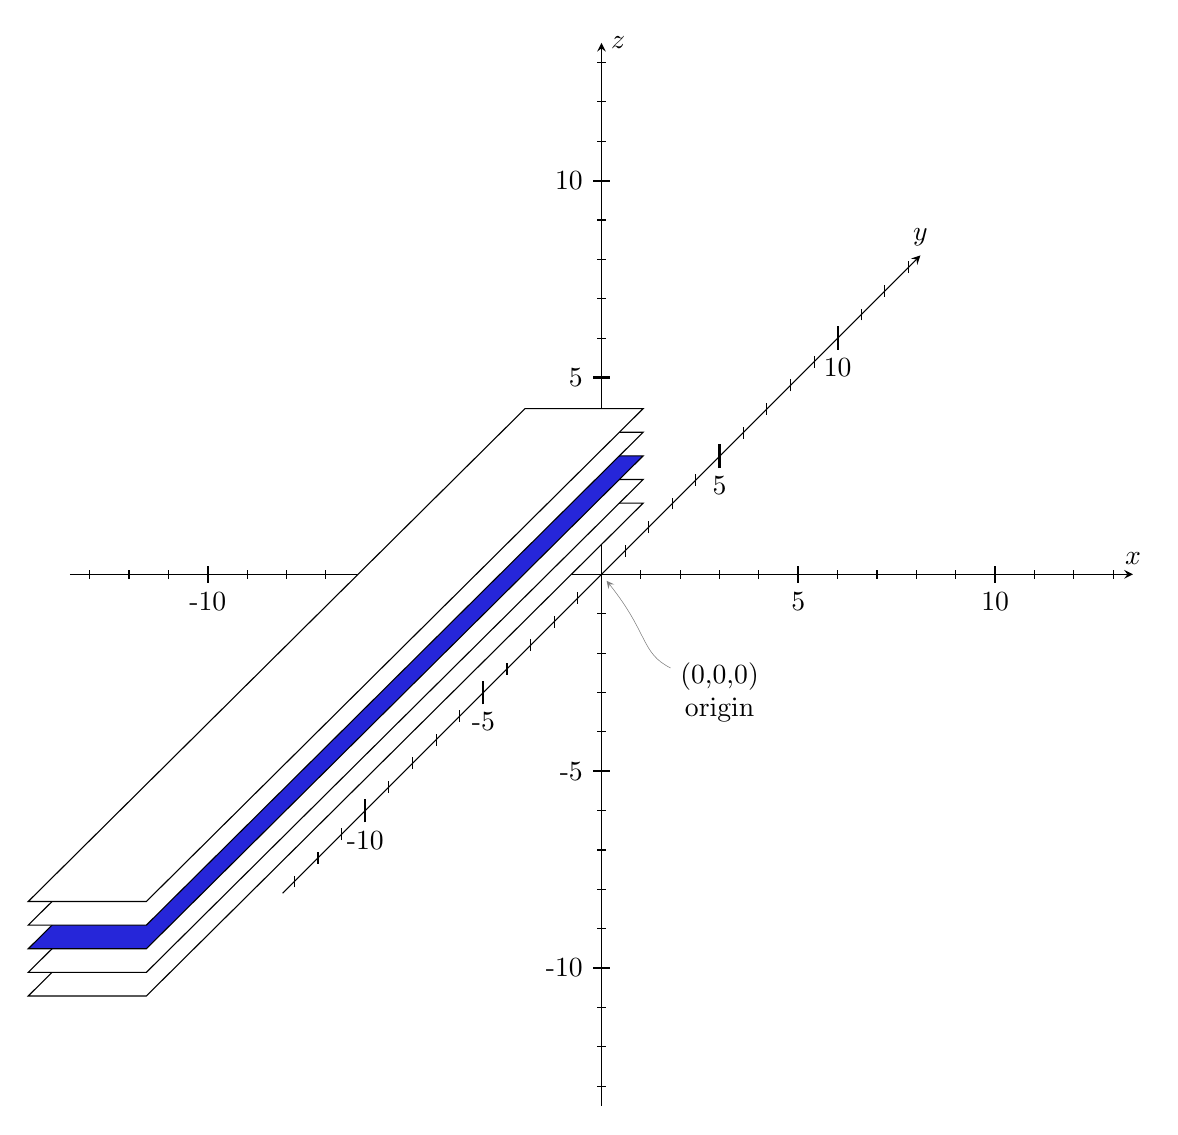
\begin{tikzpicture}[x=0.5cm,y=0.5cm,z=0.3cm,>=stealth, vector/.style={-stealth,red,thin}, 
vector guide/.style={-stealth,blue,dashed}]
% The axes
\draw[->] (xyz cs:x=-13.5) -- (xyz cs:x=13.5) node[above] {$x$};
\draw[->] (xyz cs:y=-13.5) -- (xyz cs:y=13.5) node[right] {$z$};
\draw[->] (xyz cs:z=-13.5) -- (xyz cs:z=13.5) node[above] {$y$};
% The thin ticks
\foreach \coo in {-13,-12,...,13}
{
  \draw (\coo,-1.5pt) -- (\coo,1.5pt);
  \draw (-1.5pt,\coo) -- (1.5pt,\coo);
  \draw (xyz cs:y=-0.15pt,z=\coo) -- (xyz cs:y=0.15pt,z=\coo);
}
% The thick ticks
\foreach \coo in {-10,-5,5,10}
{
  \draw[thick] (\coo,-3pt) -- (\coo,3pt) node[below=6pt] {\coo};
  \draw[thick] (-3pt,\coo) -- (3pt,\coo) node[left=6pt] {\coo};
  \draw[thick] (xyz cs:y=-0.3pt,z=\coo) -- (xyz cs:y=0.3pt,z=\coo) node[below=8pt] {\coo};
}


% The origin
\node[align=center] at (3,-3) (ori) {(0,0,0)\\\text{origin}};
\draw[->,help lines,shorten >=3pt] (ori) .. controls (1,-2) and (1.2,-1.5) .. (0,0,0);

% five planes
	\draw[fill=white!50]\plane{-0.2};
	\draw[fill=white!20]\plane{0.4};
	\draw[fill=blue!70!gray]\plane{1};
	\draw[fill=white!20]\plane{1.6};
	\draw[fill=white!20] \plane{2.2};

\end{tikzpicture}

\newpage
One important geometrical intuition we'll use over and over throughout the course is as follows. Whenever you have a surface in $\mathbb{R}^3$, think also of having a plane slice the surface at some given place, and think about the imprint left on the plane after such a slicing. We will find out later how to determine a parametrization of the curve of intersection between objects in $\mathbb{R}^3$. In the example below, a plane with a certain equation intersects a cylinder and the imprint left by this slicing is an ellipse. That ellipse essentially sit on the plane. Cases of importance involve taking planes parallel to the $xy$-plane at different $z$-elevation, slicing a  repeatedly with such planes and gathering all such imprints and looking at them.


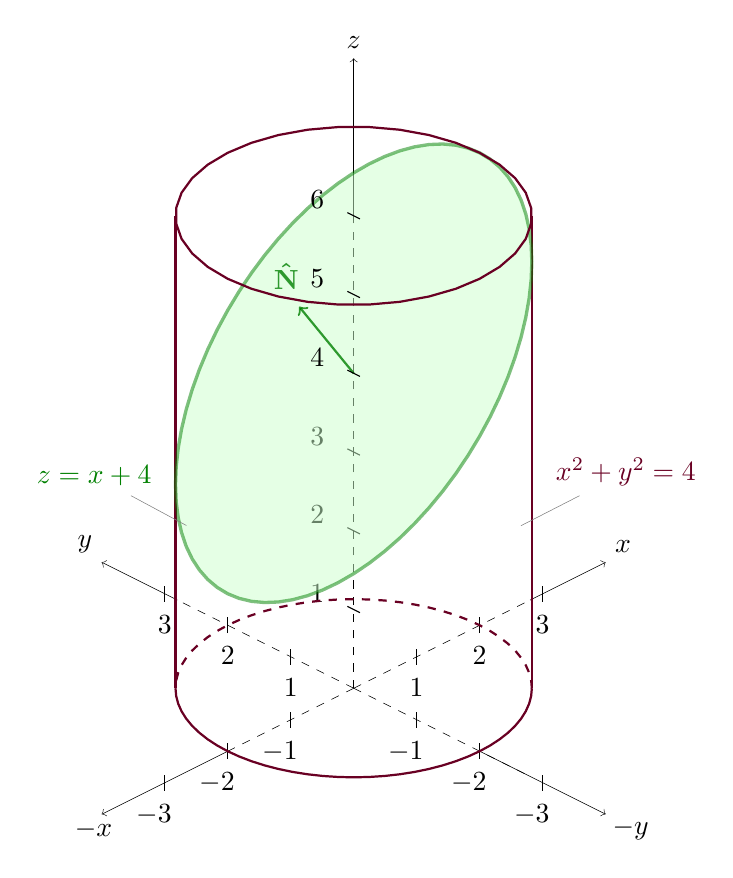
\begin{tikzpicture}[MyPersp,axis/.style={->,black,very thin}]
    \def\h{4}% Heigth of the ellipse center (on the axis of the cylinder)
    \def\a{45}% angle of the section plane with the horizontal

    \def\radius{2}
    \def\axissize{4}

    \def\clrcyl{purple!55!black}
    \def\clrplane{green}
    \def\clrplanex{\clrplane!50!black}
    \def\clrplaney{\clrplane!20!white}

    \pgfmathparse{270+\a}\edef\afirst{\pgfmathresult}
    \pgfmathparse{275+\a}\edef\asecond{\pgfmathresult}
    \pgfmathparse{450+\a}\edef\alast{\pgfmathresult}
    \pgfmathparse{90+\a}\edef\bfirst{\pgfmathresult}
    \pgfmathparse{95+\a}\edef\bsecond{\pgfmathresult}
    \pgfmathparse{270+\a}\edef\blast{\pgfmathresult}

    \draw[axis] (1.4*\radius,0,0) -- (\axissize,0,0) node[anchor=south west]{$x$};
    \draw[axis,-,dashed] (0,0,0) -- (1.4*\radius,0,0);
    \draw[axis,-,dashed] (0,0,0) -- (0,1.4*\radius,0);
    \draw[axis] (0,1.4*\radius,0) -- (0,\axissize,0) node[anchor=south east]{$y$};
    \draw[axis,-,dashed] (0,0,0) -- (0,0,\h+2);
    \draw[axis] (0,0,\h+2) -- (0,0,\h+2+.5*\axissize) node[anchor=south]{$z$};
    \draw[axis,dashed,-] (0,0,0) -- (0,-.7*\axissize,0);
    \draw[axis] (0,-\radius,0) -- (0,-\axissize,0) node[right=.125in,below=-.025in]{$-y$};
    \draw[axis,dashed,-] (0,0,0) -- (-\radius,0,0);
    \draw[axis] (-\radius,0,0) -- (-\axissize,0,0) node[below=.075in,left=-.1in]{$-x$};

    \foreach \q in {1,2,3}
    {
    \draw (\q,0,-.1) -- (\q,0,.1) node[below=.1in] {$\q$};
    \draw (-\q,0,-.1) -- (-\q,0,.1) node[below=.1in] {$\mathllap{-}\q$};
    \draw (0,\q,-.1) -- (0,\q,.1) node[below=.1in] {$\q$};
    \draw (0,-\q,-.1) -- (0,-\q,.1) node[below=.1in] {$\mathllap{-}\q$};
    }

    \foreach \q in {1,2,3}
    {
    \draw (0,-.1,\q) -- (0,.1,\q) node[left=.15in,above=-.03in] {$\q$};
    }

    \foreach \t in {135,315}%
        \draw[\clrcyl, thick] ({2*cos(\t)},{2*sin(\t)},0)
      --({2*cos(\t)},{2*sin(\t)},{2+\h});
    \draw[\clrcyl,thick] ({2*cos(\bfirst)},{2*sin(\bfirst)},0) % lower circle
    \foreach \t in {\bfirst,\bsecond,...,\blast}
            {--({2*cos(\t)},{2*sin(\t)},0)};
    \draw[\clrcyl,thick,dashed] ({2*cos(\afirst)},{2*sin(\afirst)},0) % lower circle dashed
    \foreach \t in {\afirst,\asecond,...,\alast}
            {--({2*cos(\t)},{2*sin(\t)},0)};
    \fill[\clrplaney,draw=\clrplanex,very thick,opacity=0.5]
     (2,0,\h+2) % elliptical section
        \foreach \t in {5,10,...,360}
            {--({2*cos(\t)},{2*sin(\t)},{2*cos(\t)+\h})};
    \node[pin=45:{\color{\clrcyl}$x^2+y^2=4$}] at (1.25,-1.25,2) {};
    \node[pin=135:{\color{\clrplanex}$z=x+4$}] at (-1.25,1.25,2) {};
    \draw[thick,->,\clrplanex,opacity=.8] (0,0,4) -- (0,{.5*sqrt(3)},{4+.5}) node[above=.15in,left=-.05in] {$\mathbf{\hat N}$};
    \foreach \q in {4,5,6}
    {
    \draw (0,-.1,\q) -- (0,.1,\q) node[left=.15in,above=-.03in] {$\q$};
    }

    \draw[\clrcyl, thick] (2,0,{\h+2}) % upper circle
        \foreach \t in {10,20,...,360}
            {--({2*cos(\t)},{2*sin(\t)},{\h+2})}--cycle;
\end{tikzpicture}



\newpage

Here's a similar problem just like in class. Suppose an object is being lifted as shown below. The angle $\alpha$ is $45^o$. Find the resulting total force. $Mg$ is the gravitational force. $f_R$ is the downward velocity and $T$ is the tension of the string. $N$ is the normal force.

\def\iangle{35} % Angle of the inclined plane

\def\down{-90}
\def\arcr{0.5cm} % Radius of the arc used to indicate angles

\begin{tikzpicture}[
    force/.style={>=latex,draw=blue,fill=blue},
    axis/.style={densely dashed,gray,font=\small},
    M/.style={rectangle,draw,fill=lightgray,minimum size=0.5cm,thin},
    m/.style={rectangle,draw=black,fill=lightgray,minimum size=0.3cm,thin},
    plane/.style={draw=black,fill=blue!10},
    string/.style={draw=red, thick},
    pulley/.style={thick},
]

\matrix[column sep=1cm] {
    %% Sketch
    \draw[plane] (0,-1) coordinate (base)
                     -- coordinate[pos=0.5] (mid) ++(\iangle:3) coordinate (top)
                     |- (base) -- cycle;
    \path (mid) node[M,rotate=\iangle,yshift=0.25cm] (M) {};
    \draw[pulley] (top) -- ++(\iangle:0.25) circle (0.25cm)
                   ++ (90-\iangle:0.5) coordinate (pulley);
    \draw[string] (M.east) -- ++(\iangle:1.5cm) arc (90+\iangle:0:0.25)
                  -- ++(0,-1) node[m] {};

    \draw[->] (base)++(\arcr,0) arc (0:\iangle:\arcr);
    \path (base)++(\iangle*0.5:\arcr+5pt) node {$\alpha$};
    %%

&
    %% Free body diagram of M
    \begin{scope}[rotate=\iangle]
        \node[M,transform shape] (M) {};
        % Draw axes and help lines

        {[axis,->]
            \draw (0,-1) -- (0,2) node[right] {$+y$};
            \draw (M) -- ++(2,0) node[right] {$+x$};
            % Indicate angle. The code is a bit awkward.

            \draw[solid,shorten >=0.5pt] (\down-\iangle:\arcr)
                arc(\down-\iangle:\down:\arcr);
            \node at (\down-0.5*\iangle:1.3*\arcr) {$\alpha$};
        }

        % Forces
        {[force,->]
            % Assuming that Mg = 1. The normal force will therefore be cos(alpha)
            \draw (M.center) -- ++(0,{cos(\iangle)}) node[above right] {$N$};
            \draw (M.west) -- ++(-1,0) node[left] {$f_R$};
            \draw (M.east) -- ++(1,0) node[above] {$T$};
        }

    \end{scope}
    % Draw gravity force. The code is put outside the rotated
    % scope for simplicity. No need to do any angle calculations. 
    \draw[force,->] (M.center) -- ++(0,-3) node[below] {$Mg$};
    %%



\\
};
\end{tikzpicture}

\end{document}